\documentclass[14pt,a4paper,openany]{book}
%\degree{"Доктор"} 
%\thesistitle{ПРОГНОЗИРАНЕ НА ВРЕМЕВИ РЕДОВЕ С ИЗКУСТВЕНИ НЕВРОННИ МРЕЖИ}
%\author{\href{https://www.iict.bas.bg/ipdss/p-tomov-bg.html}{инж. Петър Росенов \textsc{Томов}}}
%\supervisor{\href{http://iinf.bas.bg/bg/monov.htm}{проф. д-р Владимир Василев \textsc{Монов}}}
%\addresses{ИИКТ-БАН, ул. "акад. Георги Бончев", блок 2, етаж 5, кабинет 514, град София 1113, България} 
%\subject{02.07.20 "Комуникационни мрежи и системи" \\ 5.3 "Комуникационна и компютърна техника" \\ 5 "Технически науки"} 
%\university{\href{http://bas.bg}{Българска академия на науките}}
%\faculty{\href{http://iict.bas.bg}{Институт по информационни и комуникационни технологии}} 
%\department{\href{http://iinf.bas.bg}{Моделиране и оптимизация}}

% Добавя възможност за сензитивни хипер-връзки в самия документ.
\usepackage[pdftex, bookmarks, linktocpage]{hyperref}

% Команда с множество опции за настройка на поведението на пакета hyperref, с най-полезната опция - кирилизация на заглавията от Bookmarks в Acrobat.
\hypersetup{unicode=true, colorlinks=true, linkcolor=black, citecolor=black, urlcolor=black}

% Използване на български език.
\usepackage[T2A,T1]{fontenc}
\usepackage[utf8]{inputenc}
\usepackage[english,bulgarian]{babel}

% Използване на графика.
\usepackage[pdftex]{graphicx}

% Използване на по прецизни позиции за изображенията.
\usepackage{float}

% Използване на PDF-и за кориците.
\usepackage{pdfpages}

% Използване на хедър и футър.
\usepackage{fancyhdr}

% Използване на кавички при цитиране.
\usepackage{dirtytalk}

% Използва се за създаване на азбучен указател.
\usepackage{imakeidx}

% Използва се за листинги с програмен код.
\usepackage{listings}

% Използва се за оцветяване на клетките в таблиците.
\usepackage{xcolor,colortbl}

% Заглавие.
\title{Прогнозиране на времеви редове с изкуствени невронни мрежи}

% Автор.
\author{инж. Петър Росенов Томов}

% Директория с изображения.
\graphicspath{{images/}}

% Избор на активен език.
\selectlanguage{bulgarian}

% Текстове за декорация на страницата в горната и долната част.
\pagestyle{fancy}
\fancyhf{}
\fancyhead[LE,RO]{\thepage}
\fancyhead[RE]{Прогнозиране на времеви редове с изкуствени невронни мрежи}
\fancyhead[LO]{\thechapter}
\fancyfoot[LE,RO]{Петър Томов - ИИКТ-БАН - София - 2021}

% Дебелина на разделителните линии.
\renewcommand{\headrulewidth}{2pt}
\renewcommand{\footrulewidth}{1pt}

% Генериране на азбучен указател.
\onecolumn
\makeindex[columns=2, title=Азбучен указател, intoc]

% Подменя думата използван а за ноемрация на фрагментите програмен код.
\renewcommand{\lstlistingname}{Листинг}

% Смяна на названието за списъка от листингите.
\renewcommand{\lstlistlistingname}{Списък на листингите}

% Определя характеристиките на листигните за програмния код.
\lstset{backgroundcolor=\color{gray!30}, breaklines=true, language=r, frame=single}

% Начало на документа.
\begin{document}

% Предна корица.

\includepdf[pages={1}]{covers/front}
\thispagestyle{empty}

% Номериране на страниците със служебна информация.
\pagenumbering{roman}
\setcounter{page}{1}

% Таблица на съдържанието.
\addcontentsline{toc}{chapter}{Съдържание}
\tableofcontents

% Списък с абревиатурите и съкращенията.
\addcontentsline{toc}{chapter}{Списък на абревиатурите и съкращенията}
\chapter*{Списък на абревиатурите и съкращенията}

\begin{tabular}{ | c | c | c | c | }
\hline
\cellcolor{gray!15}Чуждоезичен термин & \cellcolor{gray!15}Съкращение & \cellcolor{gray!15}Български термин & \cellcolor{gray!15}Съкращение \\ [0.05ex] 
\hline
\hline
Differential Evolution & DE & Еволюция на разликите & ЕР \\ 
\hline
Particle Swarm Optimization & PSO & Оптимизация с рояци от частици & ОРЧ \\  
\hline
Artificial Neural Network & ANN & Изкуствена невронна мрежа & ИНМ \\  
\hline
Multi-Layer Perceptron & MLP & Многослоен перцептрон & МП \\  
\hline
& & & \\  
\hline
& & & \\  
\hline
& & & \\  
\hline
& & & \\  
\hline
& & & \\  
\hline
& & & \\  
\hline
& & & \\  
\hline
\end{tabular}

% Списък с фигурите.
\addcontentsline{toc}{chapter}{Списък на фигурите}
\listoffigures

% Списък с таблиците.
\addcontentsline{toc}{chapter}{Списък на таблиците}
\listoftables

% Списък с листингите.
\addcontentsline{toc}{chapter}{Списък на листингите}
\lstlistoflistings

% Номериране на страниците с основното изложение.
\pagenumbering{arabic}
\setcounter{page}{1}

% Отделните глави са в отделни файлове.
\addcontentsline{toc}{chapter}{Увод}
\chapter*{Увод}
\markboth{Увод}{}

Изкуствените невронни мрежи постигат изключително голяма популярност в последните пет десетилетия. Основното им предимство е възможността да възпроизвеждат нелинейни зависимости с помощта на примерни данни. Приложение намират като инструмент за класификация, разпознаване на образи и прогнозиране. При най-разпространеният вариант изкуствените невронни мрежи представляват насочени тегловни графи. Организацията е на слоеве, като информацията се предава от входния слой, към изходния слой. Най-често възлите между отделните слоеве са пълно свързани, което означава, че всеки възел е свързан с всички други възли от съседния слой. Организацията на броя слоеве и колко възли да има във всеки слой е обект на емпирично установяване и силно зависи от естеството на решаваната задача. Процесът на обучение най-често е с тренировъчни примери (обучение с учител) и целта е да се постигне такава оптимална стойност за теглата по ребрата на графа, така че изкуствената невронна мрежа максимално добре да извършва изчисленията за които е предназначена. 

\section*{Проблем}

Веднъж обучени изкуствените невронни мрежи са изключително бързо действащи. Тази тяхна характеристика ги прави особено желани в множество индустриални технически решения. Трудностите при употребата на изкуствени невронни мрежи са свързани с времето необходимо за тяхното обучение. През десетилетията са разработени множество различни алгоритми за търсене на оптимални тегла в мрежата. Двете основни направления алгоритми са градиентни (точни числени алгоритми) и евристични (най-често стохастични с въведени емпирични правила). Ускоряването на процеса по обучение е основен проблем в практическата употреба на изкуствените невронни мрежи.

\section*{Цел}

Основна цел на настоящия десертационен труд е предлагането на хибридни алгоритми за ускоряване на обучението при изкуствени невронни мрежи от тип многослоен перцептрон. Многослойният перцептрон ще бъде приложен в прогнозирането на бъдещи стойности във финансови времеви редове. 

\section*{Задачи}

За постигане на целта поставена в настоящия дисертационен труд се поставят за решаване набор от задачи. Част от задачите са с теоретичен характер и покриват подобряване на алгоритми за машинно самообучение, съчетаване (хибридизация) на алгоритмите за машинно самообучение. Другата част от задачите са с приложен характер и са свързани с прилагане на подбраните алгоритми, подходящо съчетаване на различните алгоритми (хибридизация) и практическа реализация на цялостна система са прогнозиране. Набелязаните задачи са както следва:

* Обзор на алгоритмите за обучение на изкуствени неверонни мрежи от тип многослоен перцептрон;

* Съчетаване на алгоритми за хибридно обучение на изкуствени неверонни мрежи от тип многослоен перцептрон;

* Предлагане на алгоритми за обучение на изкуствени неверонни мрежи от тип многослоен перцептрон в разпределена среда;

* Предлагане на подобрения в алгоритмите, така че да се постигне скъсяване на времето за обучение на изкуствени неверонни мрежи от тип многослоен перцептрон;

* Програмна реализация на предложените хибридни алгоритми за обучение на изкуствени неверонни мрежи от тип многослоен перцептрон;

* Извършване на сравнителен анализ за ефективността от предложеното обучение на изкуствени неверонни мрежи от тип многослоен перцептрон;

\section*{Структура}

Дисртационният труд е организиран от въведение, четири глави, заключение и приложения. Изложението е в ??? страници, ?? фигури, ?? таблици, ?? листинги и ??? литературни източника в библиографията. По дисертационния труд има ?? публикации, като ?? от тях са доклади на международни конференции, а ?? са публикувани в национални издания с международна видимост. 

В първа глава е направен обзор на широко известните алгоритми за обучение на изкуствени невронни мрежи. Разгледани са предимствата и недостатъците на точните числени алгоритми и на евристичните алгоритми. Представени са възможностите за обучение на изкуствени невронни мрежи при последователни пресмятания, паралелни пресмятания и пресмятания в разпределена среда.

Във втора глава е изложена теорията за алгоритмите при обучението на изкуствени неверонни мрежи от тип многослоен перцептрон. Направено е съчетаване между точни числени алгоритми и евристични алгоритми. Направени са предложения за реализация на хибридни алгоритми в процеса на обучението на изкуствени неверонни мрежи от тип многослоен перцептрон. 

В трета глава е представена програмната реализация на подбраните алгоритми и хибридните модификации предложени в главата за теоретичната обосновка. Представени са използваните структури от данни, обектно-ориентиран модел, релационен модел, комуникационните протоколи и графичният потребителски интерфейс. 

В четвърта глава е изложен сравнителният анализ. Описани са проведените експерименти, получените резултати и е направен кратък анализ. Определя се ефективността на предложените подобрения в алгоритмите за обучение на изкуствени неверонни мрежи от тип многослоен перцептрон.

В заключението е направено обобщение на извършените изследвания, приложен е списък с публикациите по дисертационния труд, представен е списък със забелязани цитирания, дадени са насоки за бъдещо развитие, направено е обобщение на получените резултати.


\chapter{Обзор на алгоритмите за обучение на изкуствени невронни мрежи}

В началото на 70-те години на XX век \cite{Gooijer-01} се предлагат линейни модели за прогнозиране на времеви редове – авторегресионен (Autoregressive) и плъзгащи средни (Moving Averages) \cite{Tealab-01}. При авторегресионния модел се възприема, че прогнозната стойност е линейна комбинация от стойностите в миналото. При плъзгащите средни прогнозната стойност е функция на случайни смущения - смущения, които са повлияли на времевия ред. Между двата модела е възможна комбинация под формата на авторегресионна интегрирана плъзгаща средна (Auto-Regressive Integrated Moving Average) \cite{Khashei-01}. Изкуствените неверонни мрежи се оказват един от подходите да се премине от линейност \cite{Zhang-03} към нелинейност в моделите. Трудностите при изкуствените невронни мрежи са свързани с по-големия брой параметри, които са трудни за определяне, като степен за обучение (learning rate) при обратно разпространение на грешакта или размер на скрития слой \cite{Tang-01}. Линейност и нелинейност могат да се съчетаят в хибридни реализации, базирани на плъзгащи средни и изкуствени невронни мрежи \cite{Zhang-01}. Комбинацията от линейни уравнения за постигането на разграничение при нелинейни класове се постига и чрез машина с поддържащи вектори (Support Vector Machines) \cite{Kyoung-jae-01}. Машините с поддържащи вектори се явяват подобрение на изкуствените невронни мрежи обучавани по правилото за обратно разпространение на грешката. Времето за обучение се намалява, докато достоверността на прогнозите се увеличава \cite{Tay-01}. Ефективността на машините с поддържащи вектори може да се подобри, когато се използват алгоритми за адаптиране на параметрите \cite{Cao-01}. При времеви редове с ясно изразен тренд и сезонност, премахването им може да подобри възможностите за генериране на прогноза \cite{Zhang-02}.


\chapter{Предложение за алгоритми при обучение на изкуствени невронни мрежи}

\section{Бърз прототип на LibreOffice Calc с еволюция на разликите и оптимизация с рояк от частици}

Процесът по търсенето на оптимални тегла в изкуствена невронна мрежа от тип трислоен перцептрон много нагледно може да бъде демонстриран с бърз прототип в софтуерния пакет LibreOffice Calc. За осъществяване на прототипирането моделът на изкуствената невронна мрежа бива разгърнат в двузимерната равнина от клетки на електронната таблица. Търсенето на оптимални стойности за теглата в мрежата се постига чрез вградения в LibreOffice Calc модул за оптимизация наречен Solver (Фиг. \ref{fig001}).

\begin{figure}[h]
  \centering
  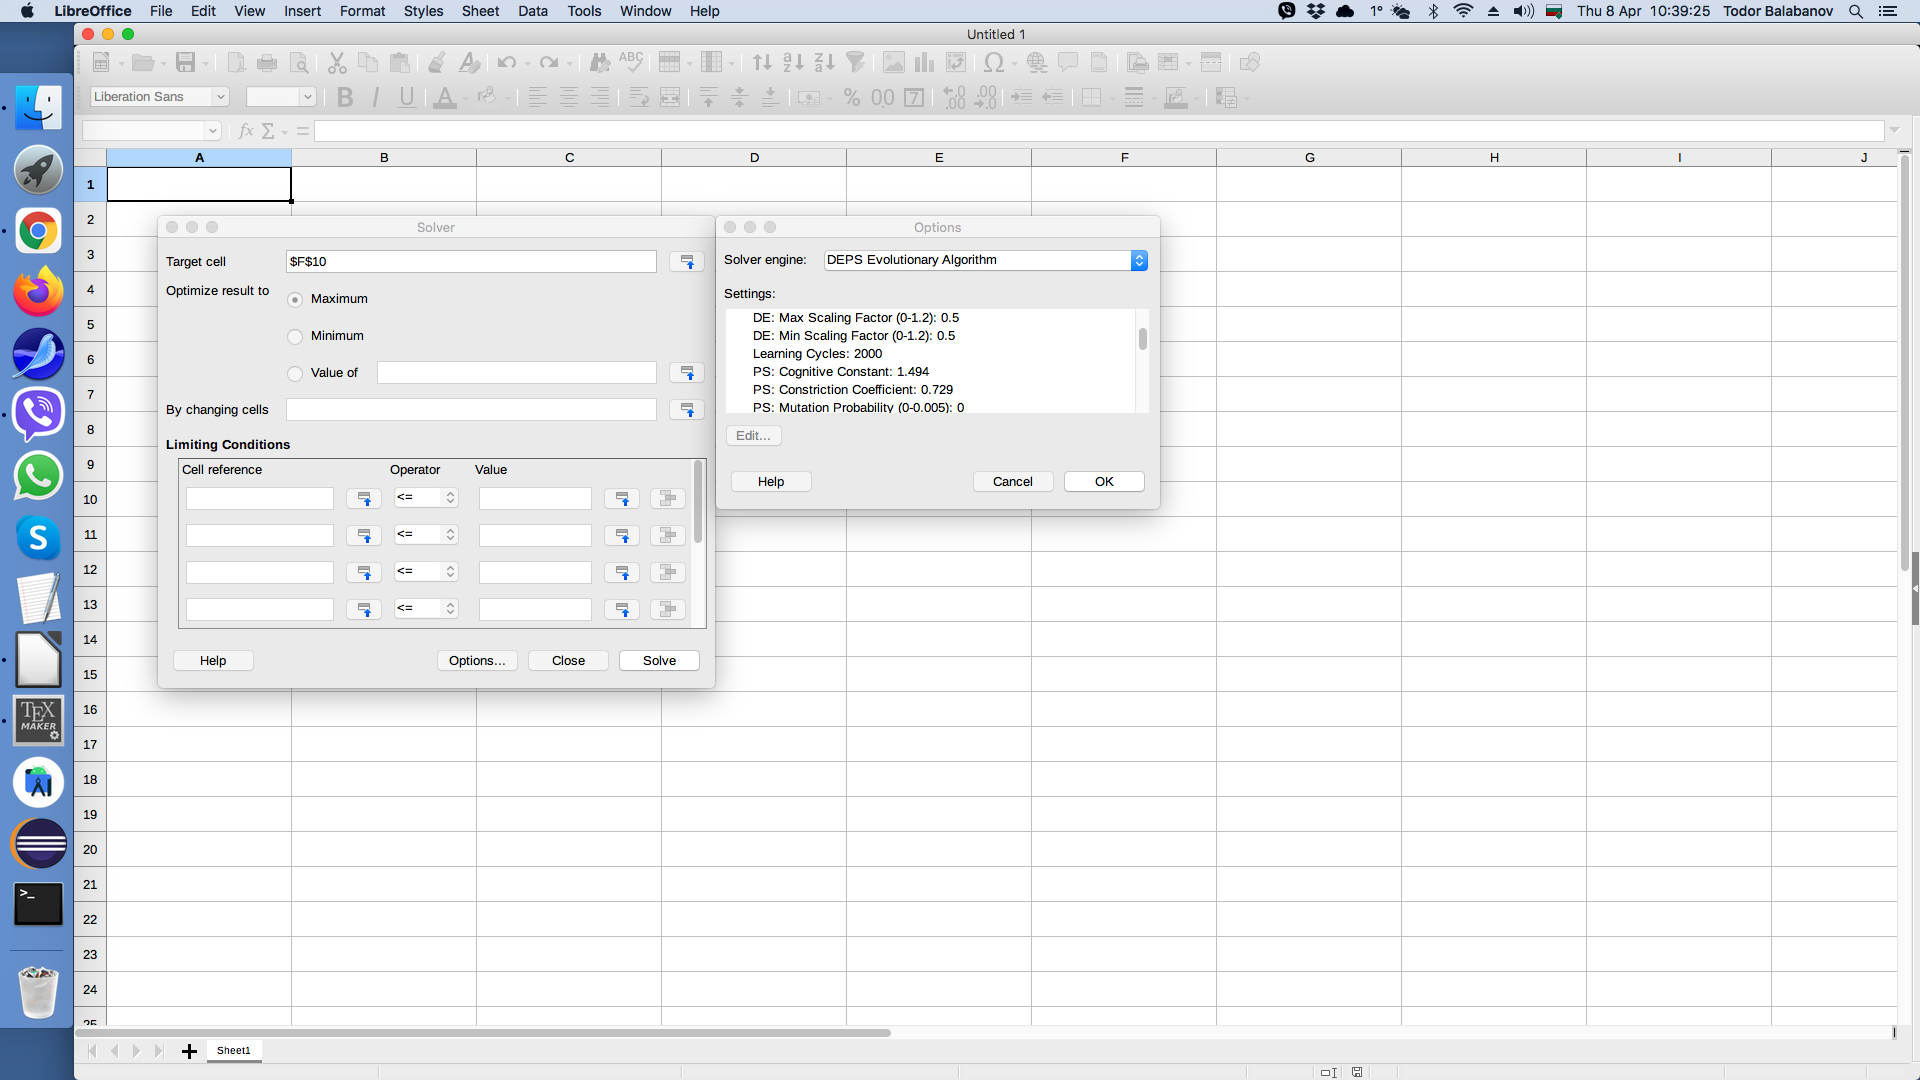
\includegraphics[width=1.0\linewidth]{fig001.png}
  \caption{Модул за оптимизация в LibreOffice Calc}
\label{fig001}
\end{figure}

За нелинейна оптимизация модулът прилага алгоритмите за еволюция на разликите и оптимизация с рояк от частици. Двата алгоритъма се прилагат в хибридна комбинация, като с предварително дефинирана вероятност е определено колко често ще бъде активиран всеки от тях. Модулът се настройва за клетка, чиято оптимална стойност ще бъде търсена (максимум, минимум или конкретно число). Също така, задава се и регионът от клетки, които подлежат на промяна в процеса по оптимизация. Като клетка в която ще се търси минимум при бързото протитипиране се избира общата средно-квадратична грешка допусната от изкуствената невронна мрежа. Регионът от клетки за оптимизация съдържа теглата използевани в изкуствената невронна мрежа. 

\begin{figure}[h]
  \centering
  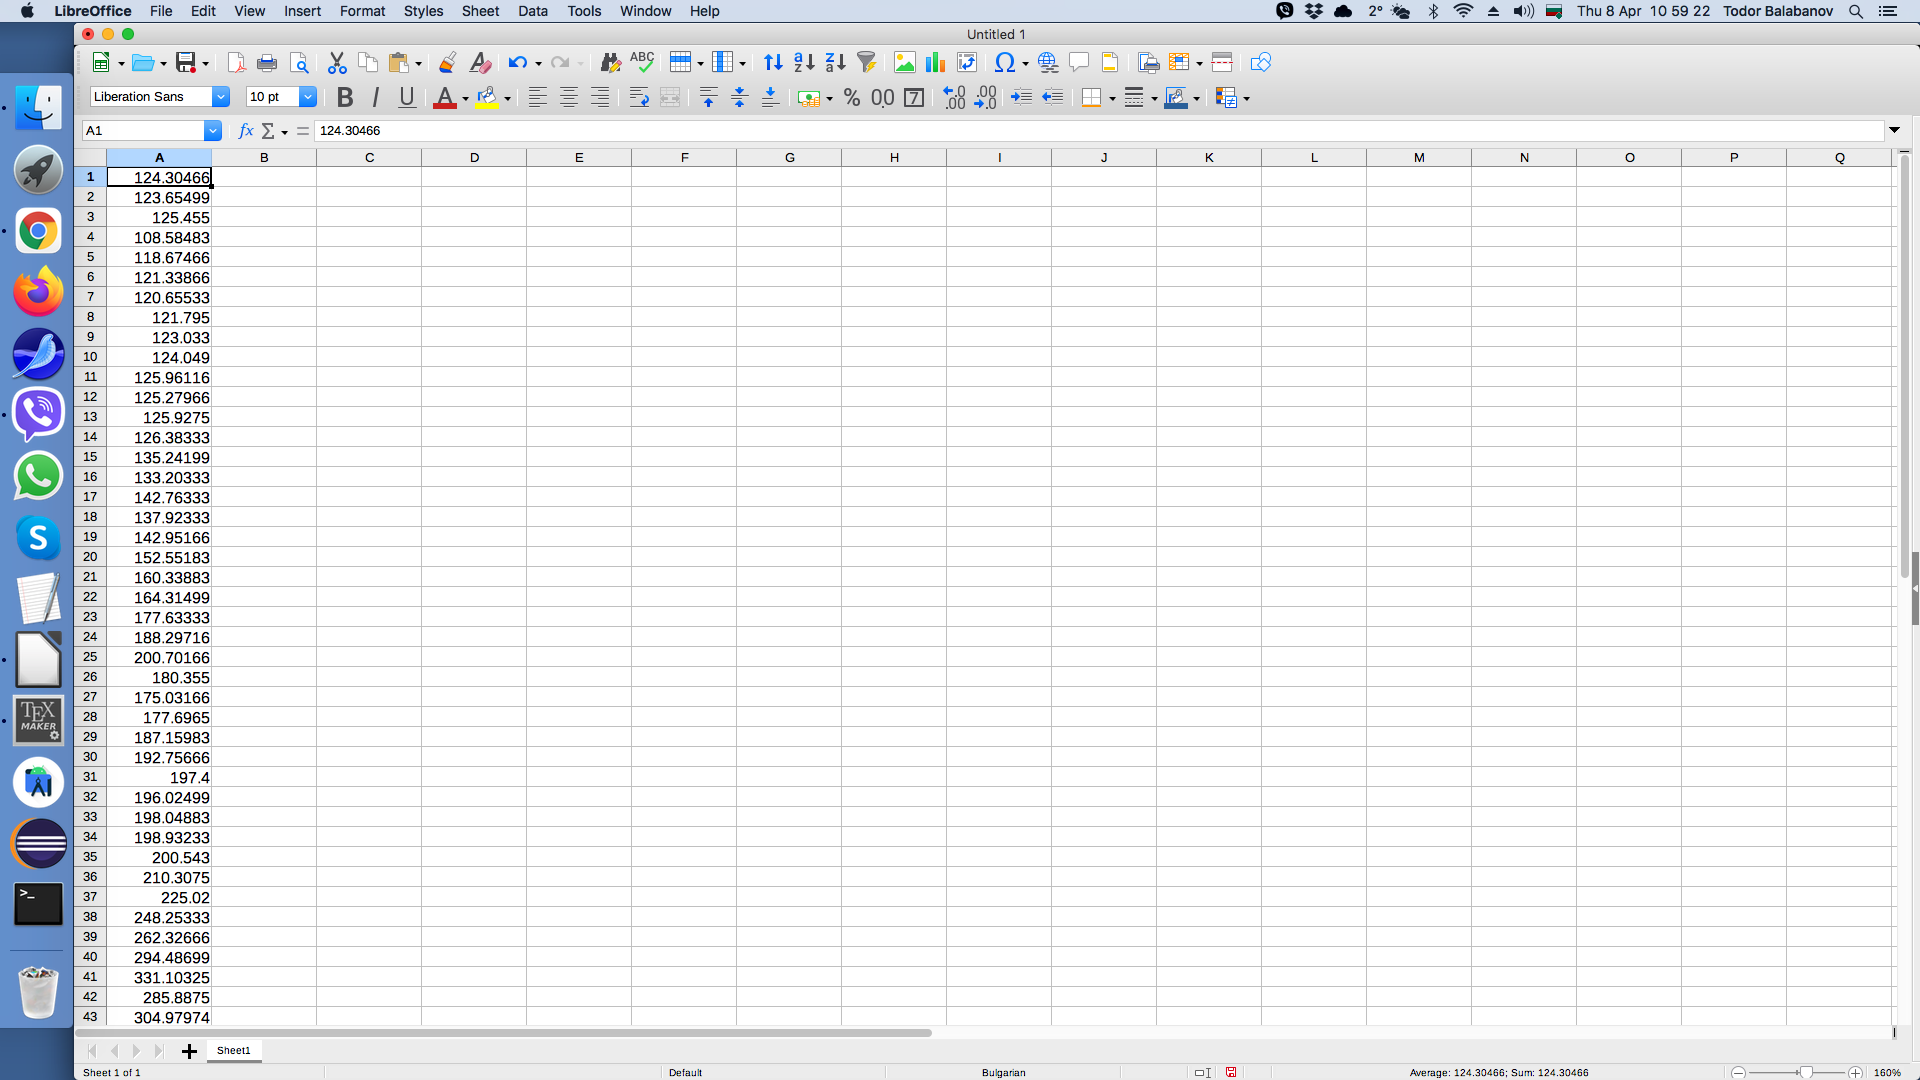
\includegraphics[width=1.0\linewidth]{fig002.png}
  \caption{Стойности на Bitcoin виртуалната валута}
\label{fig002}
\end{figure}

Като множество данни се използват стойностите на Bitcoin виртуалната валута (Фиг. \ref{fig002}), на дневна база, за няколко години назад. Моделът за прогнозиране се основава на нелинейна авторегресия. Това означава, че на входа на мрежата се подават мащабирани минали стойности от времевия ред, а на изхода на мрежата се очакват мащабирани прогнозни стойности. 

\begin{figure}[h]
  \centering
  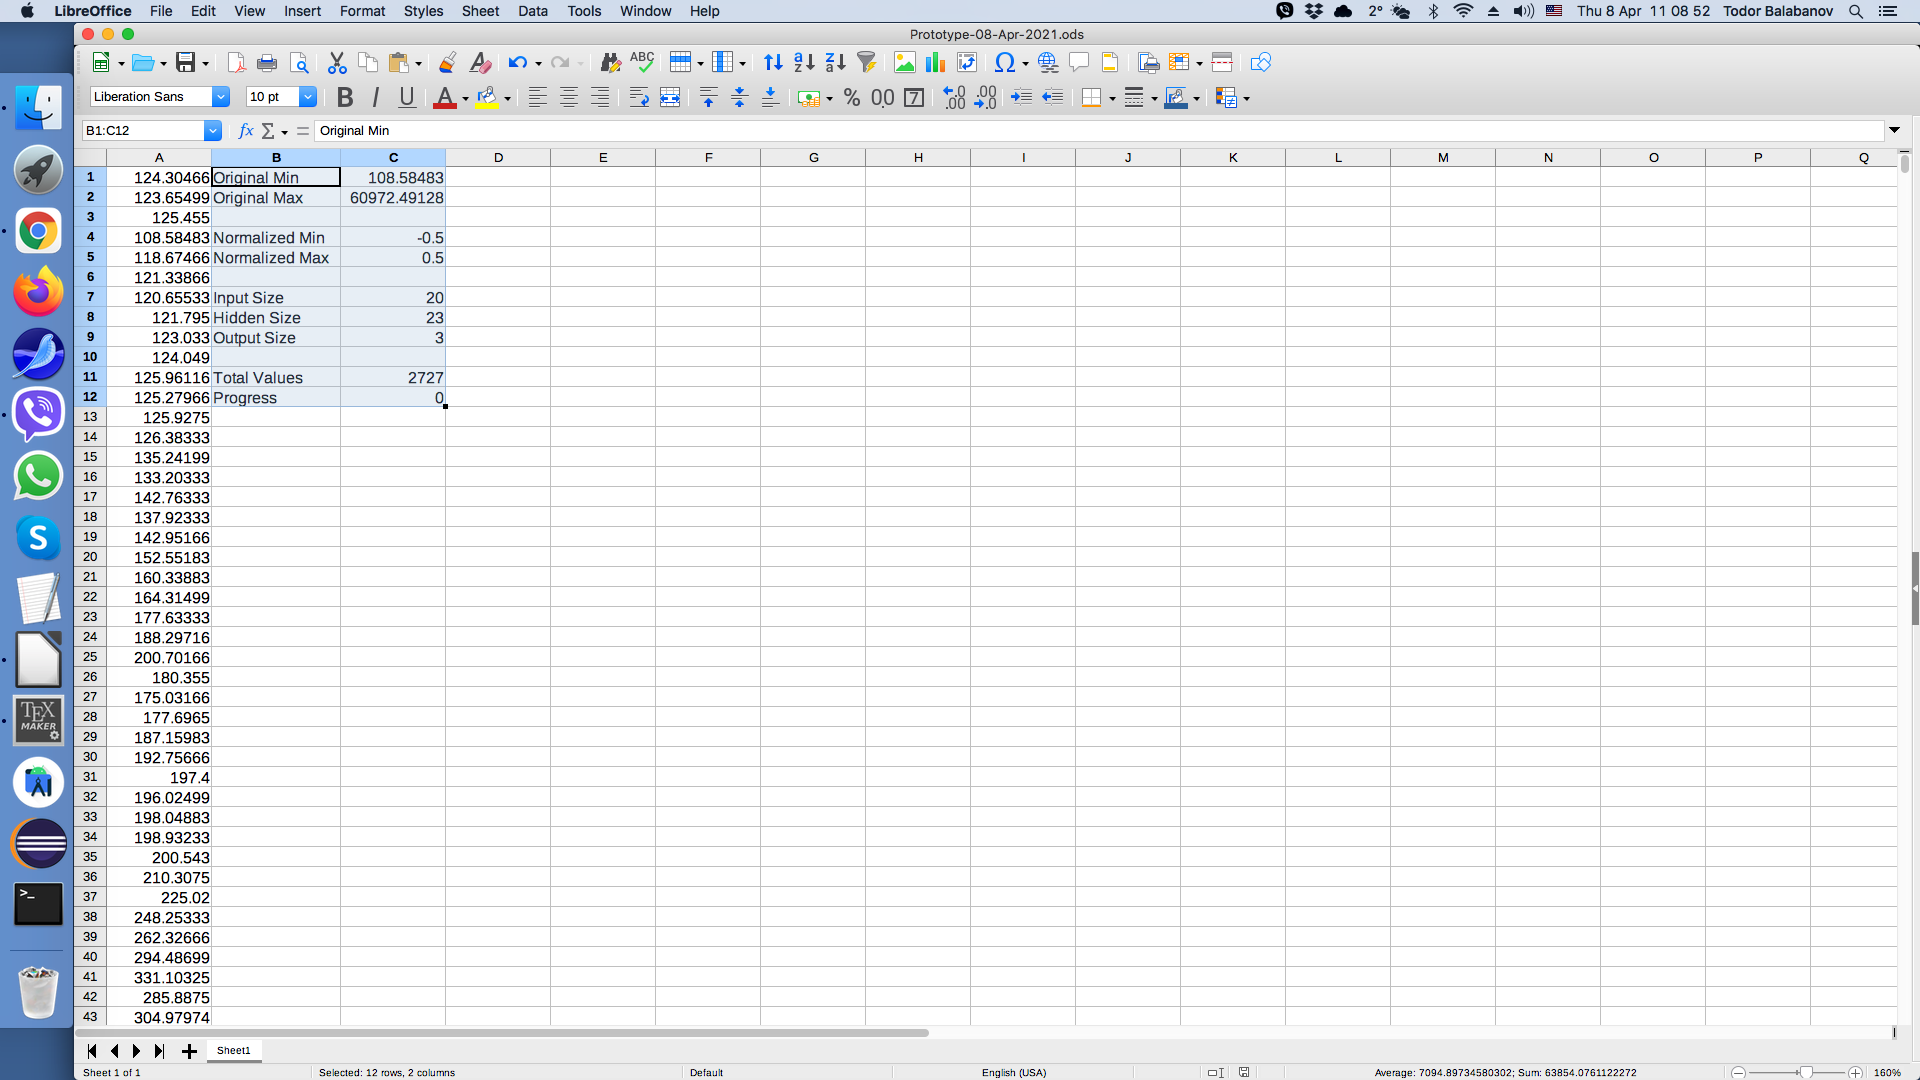
\includegraphics[width=1.0\linewidth]{fig003.png}
  \caption{Параметри на трислойната изкуствена невронна мрежа}
\label{fig003}
\end{figure}

След подбора на времеви ред следва избор на параметрите с които ще бъде напревен модела на трислойната изкуствена невронна мрежа (Фиг. \ref{fig003}). За целите на линейното мащабиране първо се намират най-малката и най-голямата стойност в оригиналния времеви ред, чрез формули в LibreOffice Calc: $=MIN(A:A)$ и $=MAX(A:A)$. Тъй като приложената прагова функция е хиперболичен тангенс, диапазона за мащабирания времеви ред е избран от -0.5 до +0.5. Умишлено се избягва мащабиране до асимптотичните стойности от -1.0 до +1.0, тъй като такова мащабиране много би увеличило стойностите на междинните пресмятания, а и не би дало възможност да се прогнозират по-малки или по-големи стойности от вече известните в оригиналния времеви ред. Топологията на мрежата се избира експериментално, като изходния слой има размер, според това колко стойности в бъдещето е желателно да се предсказват. Размера на входния слой се определя експериментално. За размера на скрития слой има различни емпирични правила, като най-популярното е скритият слой да бъде половината от сумата на размерите имащи входния и изходния слой. Съществуват адаптивни алгоритми, които чрез проби и грешки да определят топологията на мрежата, но в това бързо прототипиране тези алгоритми не се прилагат. 

Общият брой стойности в оригиналния времеви ред се определят с формула в LibreOffice Calc: $=COUNT(A:A)$. Тъй като процеса по „разгръщането“ на модела е относително бавен, то се добавя клетка в която да се проследява напредъка от Python скрипта в „разгръщането“. LibreOffice Calc позволява изпълнението на макроси, като се поддържат няколко програмни езика. Програмният език Python е изключително популярен в сферата на машинното самообучение и дава изключително големи възможности за частична автоматизация в програмите на LibreOffice.

След мащабирането на оригиналния времеви ред се формират тренировъчните примери, като за вход се вземат стойности преди условния момент $t_0$, а за очакван изход стойности след условния момент $t_0$ (условно разделяне на минало и бъдеще).

\begin{lstlisting}[caption=Мащабиране на оригиналния времеви ред, language=Python, basicstyle=\tiny, label=listing001]
    ''' Scale input. '''
    for t in range(1, total_values + 1):
        sheet.getCellRangeByName("E" + str(t)).setValue(sheet.getCellRangeByName("$C$4").getValue() + 
        (sheet.getCellRangeByName("$C$5").getValue() - sheet.getCellRangeByName("$C$4").getValue()) * ((sheet.getCellRangeByName("A" + str(t)).getValue() - 
        sheet.getCellRangeByName("$C$1").getValue()) / (sheet.getCellRangeByName("$C$2").getValue() - sheet.getCellRangeByName("$C$1").getValue())))
\end{lstlisting}

В листинг \ref{listing001} се демонстрира линейното мащабиране, като за извършване на изчисленията се използват установените минимални и максимални стойности (Фиг. \ref{fig004}). 

\begin{figure}[h]
  \centering
  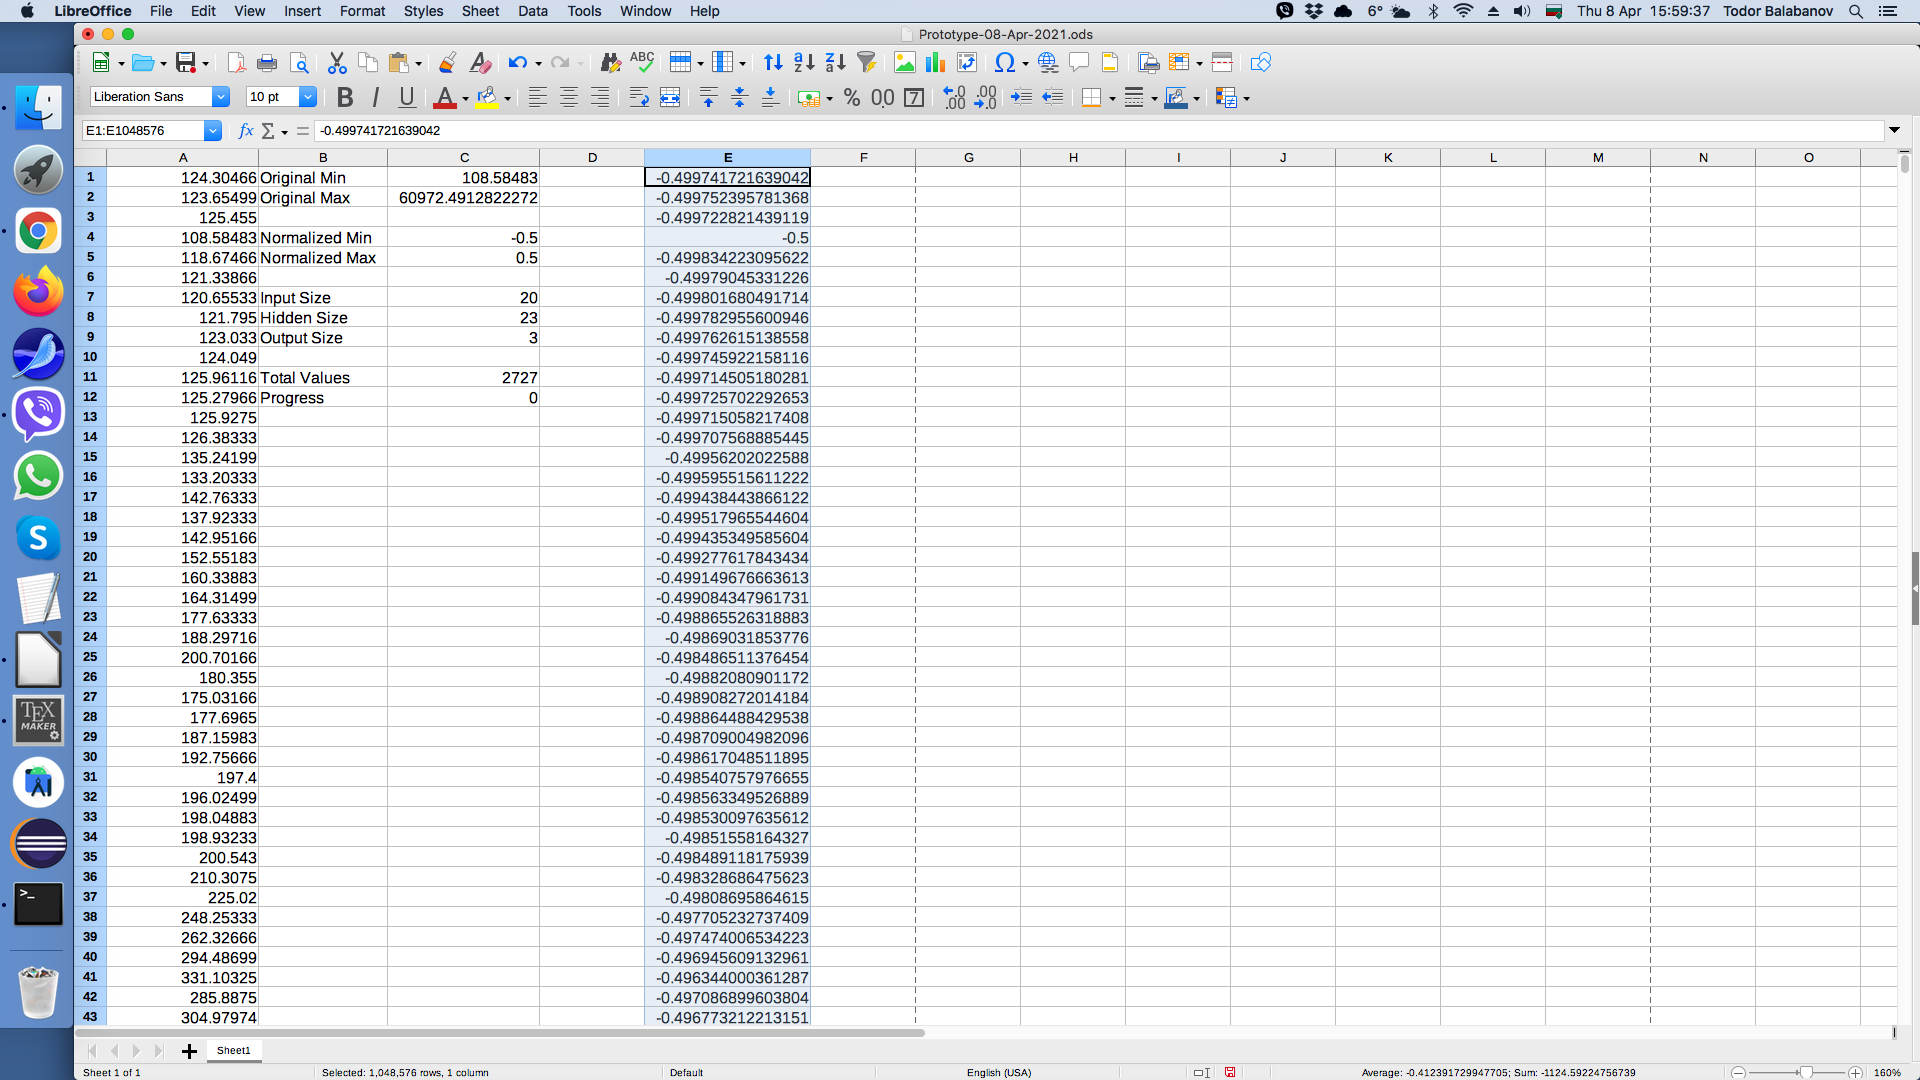
\includegraphics[width=1.0\linewidth]{fig004.png}
  \caption{Резултат от мащабирането на времевия ред}
\label{fig004}
\end{figure}

На всеки слой в изкуствената невронна мрежа се добавя по един допълнителен неврон (Листинг \ref{listing002}), постоянно емитиращ единична стойност (отместване или от английски език bias).

\begin{lstlisting}[caption=Неврони емитиращи постоянно единичен сигнал, language=Python, basicstyle=\tiny, label=listing002]
        ''' Setup biases. '''
        sheet.getCellRangeByName("G" + str(x)).setValue(1)
        sheet.getCellRangeByName("G" + str(x)).CellBackColor = (255 << 16 | 255 << 8 | 0)
        sheet.getCellRangeByName("H" + str(x)).setValue(1)
        sheet.getCellRangeByName("H" + str(x)).CellBackColor = (255 << 16 | 255 << 8 | 0)
        sheet.getCellRangeByName("I" + str(x)).setValue(1)
        sheet.getCellRangeByName("I" + str(x)).CellBackColor = (255 << 16 | 255 << 8 | 0)
        sheet.getCellRangeByName("J" + str(x)).setValue(1)
        sheet.getCellRangeByName("J" + str(x)).CellBackColor = (255 << 16 | 255 << 8 | 0)
\end{lstlisting}

Мащабираният времеви ред бива „разбит“ условно на „минали“ стойности и „бъдещи“ стойности. Миналите стойности стават входни сигнали за изкуствената невронна мрежа (Листинг \ref{listing003}).

\begin{lstlisting}[caption=Формиране на входния слой, language=Python, basicstyle=\tiny, label=listing003]
        ''' Input data loading. '''
        for i in range(1, input_size + 1):
            sheet.getCellRangeByName("G" + str(x + i)).setValue(sheet.getCellRangeByName("E" + str(t + i)).getValue())
            sheet.getCellRangeByName("G" + str(x + i)).CellBackColor = (255 << 16 | 0 << 8 | 0)
\end{lstlisting}

По аналогичен начин, будещите стойности се зареждат като очакван изход от изкуствената невронна мрежа (Листинг \ref{listing004}).

\begin{lstlisting}[caption=Очакван изход от мрежата, language=Python, basicstyle=\tiny, label=listing004]
        ''' Expected data loading. '''
        for e in range(1, output_size + 1):
            sheet.getCellRangeByName("J" + str(x + e)).setValue(sheet.getCellRangeByName("E" + str(t + e + input_size)).getValue())
            sheet.getCellRangeByName("J" + str(x + e)).CellBackColor = (0 << 16 | 127 << 8 | 0)
\end{lstlisting}

Стойностите във възлите на скрития слой са резултат от пресмятане на входните сигнали и текущите стойности на теглата в мрежата (Листинг \ref{listing005}). 

\begin{lstlisting}[caption=Стойности на скрития слой при правия пас, language=Python, basicstyle=\tiny, label=listing005]
        ''' Setup hidden layer. '''
        wih = 1
        for h in range(1, hidden_size + 1):
            sum = ""
            for i in range(0, input_size + 1):
                sum = sum + "G" + str(x + i) + "*Q" + str(wih)
                wih = wih + 1
                if i < input_size:
                    sum = sum + " + "
            sheet.getCellRangeByName("H" + str(x + h)).setFormula("=TANH( " + sum + " )")
            sheet.getCellRangeByName("H" + str(x + h)).CellBackColor = (0 << 16 | 0 << 8 | 255)
\end{lstlisting}

На свой ред, стойностите в изходния слой са резултат от пресмятане на сигналите в скрития слой и текущите стойности на теглата в мрежата (Листинг \ref{listing006}).

\begin{lstlisting}[caption=Стойности на изходния слой при правия пас, language=Python, basicstyle=\tiny, label=listing006]
        ''' Setup output layer. '''
        who = 1
        for o in range(1, output_size + 1):
            sum = ""
            for h in range(0, hidden_size + 1):
                sum = sum + "H" + str(x + h) + "*S" + str(who)
                who = who + 1
                if h < hidden_size:
                    sum = sum + " + "
            sheet.getCellRangeByName("I" + str(x + o)).setFormula("=TANH( " + sum + " )")
            sheet.getCellRangeByName("I" + str(x + o)).CellBackColor = (0 << 16 | 255 << 8 | 0)
\end{lstlisting}

Стойностите в изходния слой, спрямо очакваните стойности дават грешката, която изкуствената невронна мрежа допуска за конкретния тренировъчен пример (Листинг \ref{listing007}).

\begin{lstlisting}[caption=Стойност на грешката допусната от мрежата за конкретния пример, language=Python, basicstyle=\tiny, label=listing007]
        ''' Network output error. '''
        for r in range(1, output_size + 1):
            sheet.getCellRangeByName("K" + str(x + r)).setFormula("= (J" + str(x + r) + "-I" + str(x + r) + ") * (J" + str(x + r) + "-I" + str(x + r) + ")")
            sheet.getCellRangeByName("K" + str(x + r)).CellBackColor = (0 << 16 | 255 << 8 | 255)
\end{lstlisting}

Така описаното разполагане по клетките на листа в електронната таблица се повтаря многократно, така че да се появи фрагмент за всеки тренировъчен пример. Фрагментът съдържа входен слой, скрит слой, изходен слой и очаквани на изхода стойности (Фиг. \ref{fig005}).

\begin{figure}[h]
  \centering
  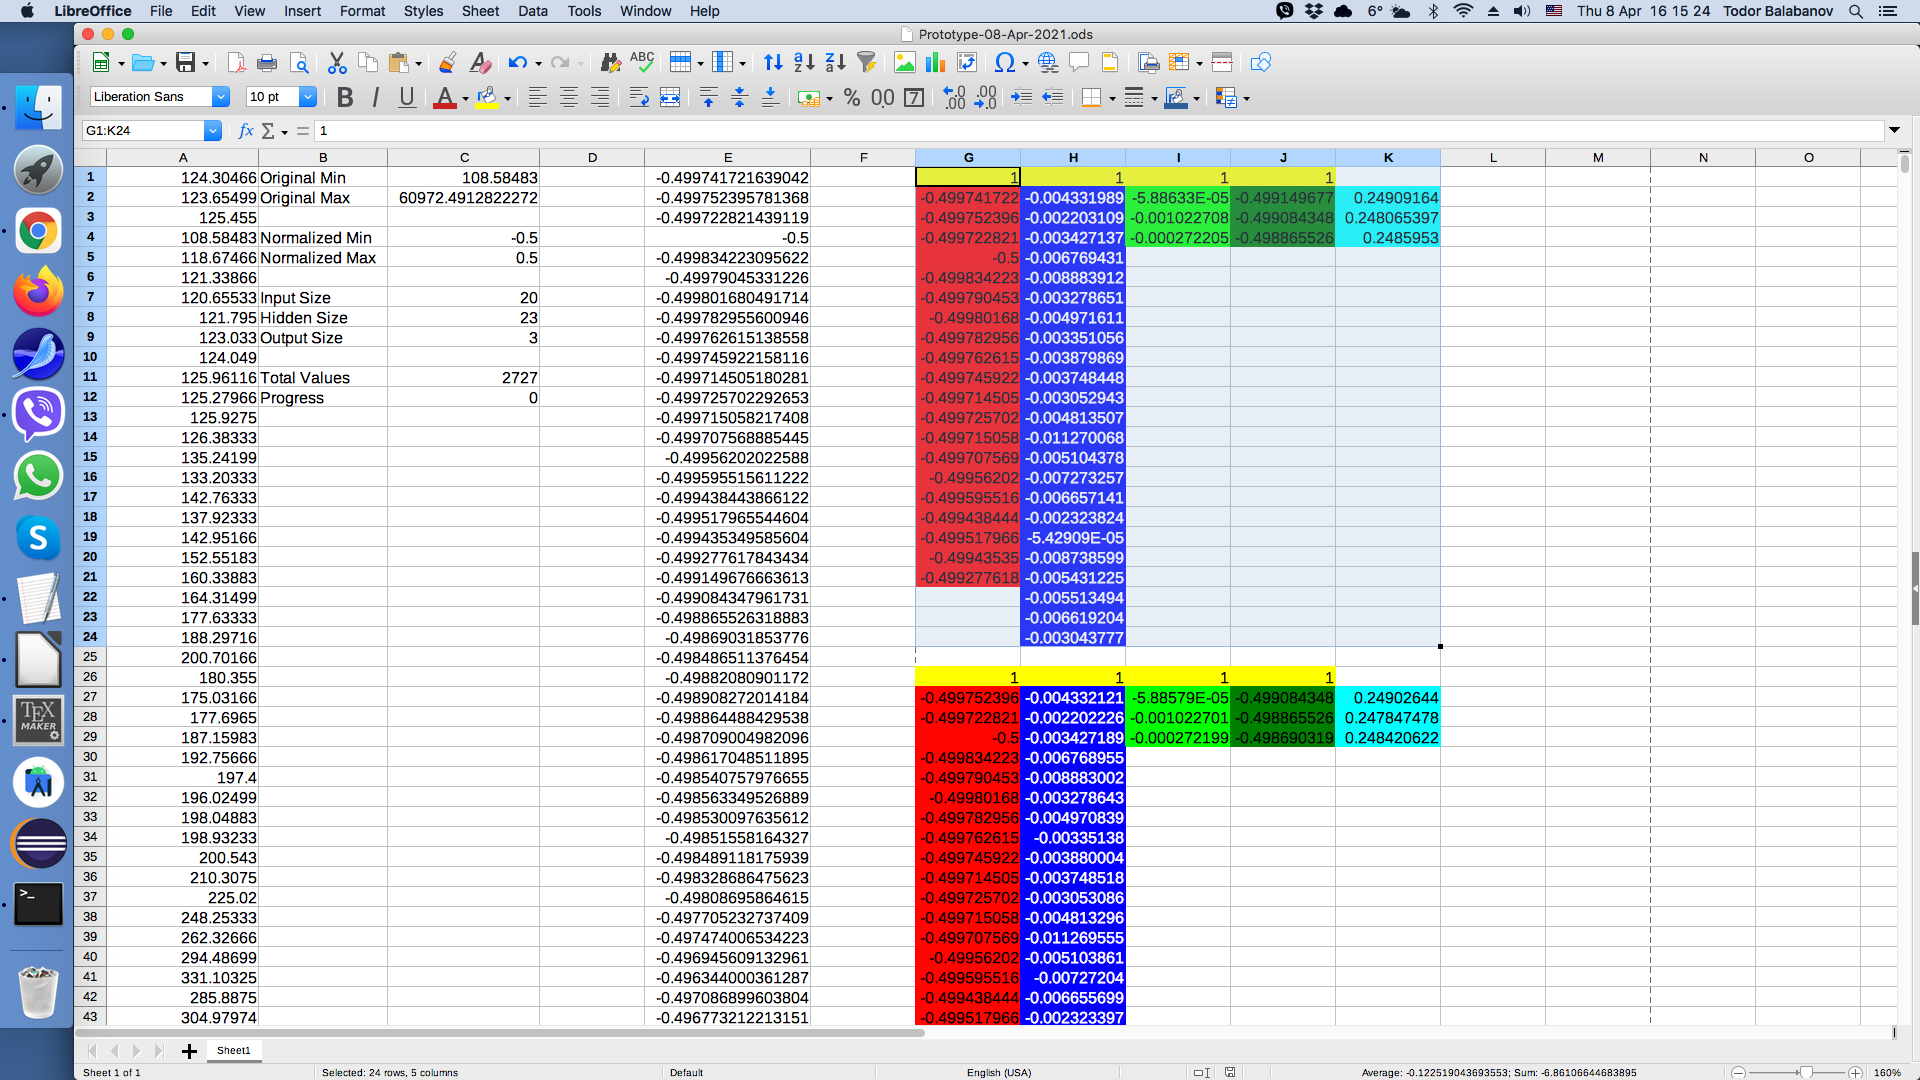
\includegraphics[width=1.0\linewidth]{fig005.png}
  \caption{Фрагменти за тренировъчните примери}
\label{fig005}
\end{figure}

Общата грешка, допусната от мрежата при всички тренировъчни примери е на базата на средно-квадратична грешка (Листинг \ref{listing008}).

\begin{lstlisting}[caption=Обща средно-квадратична грешка на мрежата, language=Python, basicstyle=\tiny, label=listing008]
    ''' Network total error. '''
    sheet.getCellRangeByName("M1").setFormula("= SQRT( SUM(K:K) / COUNT(K:K) )")
    sheet.getCellRangeByName("M1").CellBackColor = 0
\end{lstlisting}

Два региона клетки в листа на електронната таблица се определят за стойностите на теглата в мрежата, както и обратно мащабиране към оригиналните стойности (Листинг \ref{listing009}).

\begin{lstlisting}[caption=Определяне на региони за теглата на мрежата, language=Python, basicstyle=\tiny, label=listing009]
    ''' Setup hidden layer weights. '''
    wih = 1
    for h in range(2, hidden_size + 2):
        for i in range(1, input_size + 2):
            sheet.getCellRangeByName("Q" + str(wih)).CellBackColor = (255 << 16 | 0 << 8 | 255)
            wih = wih + 1
        
    ''' Setup output layer weights. '''
    who = 1
    for o in range(2, output_size + 2):
        for h in range(1, hidden_size + 2):
            sheet.getCellRangeByName("S" + str(who)).CellBackColor = (255 << 16 | 0 << 8 | 255)
            who = who + 1

        sheet.getCellRangeByName("U" + str(o)).setFormula("=$C$1 + ($C$2 - $C$1) * ((T" + str(o) + " - $C$4) / ($C$5 - $C$4))")
        sheet.getCellRangeByName("U" + str(o)).CellBackColor = (0 << 16 | 127 << 8 | 0)
\end{lstlisting}

За да не се блокира графичния потребителски интерфейс, „разгръщането“ на модела на изкуствената невронна мрежа се извършва в отделна нишка (Листинг \ref{listing010}).


\begin{lstlisting}[caption=Изпълнение с отделна нишка, language=Python, basicstyle=\tiny, label=listing010]
def BuildAnnModel():
    thread = Thread(target=ThreadWorker, args=(XSCRIPTCONTEXT.getDesktop(),))
    thread.start()
\end{lstlisting}


\chapter{Глава 3 - }
\chapter{Глава 4 - }
\addcontentsline{toc}{chapter}{Заключение}
\chapter*{Заключение}

\newpage
\section*{Резюме на получените резултати}

\subsection*{Научно-приложни резултати}

\subsection*{Приложни резултати}

\newpage
\section*{Насоки за бъдещи изследвания}

\newpage
\section*{Публикации по темата на дисертационния труд}

\newpage
\section*{Забелязани цитирания}

\newpage
\section*{Декларация за оригиналност на резултатите}

\vspace{1cm}

Декларирам, че дисертацията съдържа оригинални резултати, получени при проведени от мен, научни изследвания с подкрепата и съдействието на научния ми ръководител.

Резултатите, които са получени, описани и/или публикувани от други учени, са коректно и подробно цитирани в библиографията.

Настоящият дисертационен труд не е прилаган за придобиване на научна степен в друго висше училище, университет или научен институт.

\vspace{2cm}

\begin{tabular}{ c c c c }
Дата: & .......................................... & Подпис: & .......................................... \\ 
& гр. София & & / Петър Томов / \\  
\end{tabular}


% Списък с използвана литература и източници на информация.
\addcontentsline{toc}{chapter}{Библиография}
%\chapter*{Библиография}

\begin{thebibliography}{99.}

\bibitem{Alba-01} Alba, E., Tomassini, M.: Parallelism and evolutionary algorithms. IEEE Transactions on Evolutionary Computation, vol. 6, no. 5, 443--462, 2002. ISSN 1089-778X DOI 10.1109/TEVC.2002.800880

\bibitem{Basheer-01} Basheer, I., Hajmeer, M.: Artificial neural networks: fundamentals, computing, design, and application. Journal of Microbiological Methods, vol. 43, no. 1, 3--31, 2000. ISSN 0167-7012 DOI 10.1016/S0167-7012(00)00201-3

\bibitem{Beyer-02} Beyer, H.: Evolutionary algorithms in noisy environments: theoretical issues and guidelines for practice. Computer Methods in Applied Mechanics and Engineering, vol. 186, no. 2-4, 239--267, 2000. ISSN 0045-7825 DOI 10.1016/S0045-7825(99)00386-2

\bibitem{Beyer-01} Beyer, H., Schwefel, H., Wegener, I.: How to analyse evolutionary algorithms. Theoretical Computer Science, vol. 287, no. 1, 101--130, 2002. ISSN 0304-3975 DOI 10.1016/S0304-3975(02)00137-8

\bibitem{Bilbao-01} Bilbao, I., Bilbao, J.: Overfitting problem and the over-training in the era of data: Particularly for Artificial Neural Networks. Proceedings of Eighth International Conference on Intelligent Computing and Information Systems, 173--177, 2017. ISBN 978-1-5386-0822-7 DOI 10.1109/INTELCIS.2017.8260032

\bibitem{Bing-01} Bing, Y., Hao, J., Zhang, S.: Stock Market Prediction Using Artificial Neural Networks. Advanced Engineering Forum, vol. 6-7, 1055--1060, 2012. ISSN 2234-991X DOI 10.4028/www.scientific.net/AEF.6-7.1055

\bibitem{Bontempi-01} Bontempi, G., Ben Taieb, S., Le Borgne Y.: Machine Learning Strategies for Time Series Forecasting. Lecture Notes in Business Information Processing, vol 138, 62--77, 2013. ISBN 978-3-642-36317-7 DOI 10.1007/978-3-642-36318-4\_3

\bibitem{Cao-01} Cao, L., Tay, F.: Support vector machine with adaptive parameters in financial time series forecasting. IEEE Transactions on Neural Networks, vol. 14, no. 6, 1506--1518, 2003. ISSN 1045-9227 DOI 10.1109/TNN.2003.820556

\bibitem{Cao-02} Cao, J., Li, Z., Li, J.: Financial time series forecasting model based on CEEMDAN and LSTM. Physica A: Statistical Mechanics and its Applications, vol. 519, 127--139, 2019. ISSN 0378-4371 DOI 10.1016/j.physa.2018.11.061

\bibitem{Caponetto-01} Caponetto, R., Fortuna, L., Fazzino, S., Xibilia, M.: Chaotic sequences to improve the performance of evolutionary algorithms. IEEE Transactions on Evolutionary Computation, vol. 7, no. 3, 289--304, 2003. DOI 10.1109/TEVC.2003.810069

\bibitem{Chandwani-01} Chandwani, V., Agrawal, V., Nagar, R.: Modeling slump of ready mix concrete using genetic algorithms assisted training of Artificial Neural Networks. Expert Systems with Applications, vol. 42, no. 2, 885--893, 2015. ISSN 0957-4174 DOI 10.1016/j.eswa.2014.08.048

\bibitem{Chen-01} Chen, Y., Yang, B., Dong, J., Abraham. A.: Time-series forecasting using flexible neural tree model. Information Sciences, vol. 174, no. 3--4, 219--235, 2005. ISSN 0020-0255 DOI 10.1016/j.ins.2004.10.005

\bibitem{Chen-02} Chen, J., Do, Q., Hsieh, H.: Training Artificial Neural Networks by a Hybrid PSO-CS Algorithm. Algorithms, vol. 8, no. 2, 292--308, 2015. ISSN 1999-4893 DOI 10.3390/a8020292

\bibitem{Cheng-01} Cheng, R., He, C., Jin, Y., Yao, X.: Model-based evolutionary algorithms: a short survey. Complex \& Intelligent Systems, vol. 4, 283--292, 2018. ISSN 2198-6053 DOI 10.1007/s40747-018-0080-1

\bibitem{Coello-01} Coello, C.: Theoretical and numerical constraint-handling techniques used with evolutionary algorithms: a survey of the state of the art. Computer Methods in Applied Mechanics and Engineering, vol. 191, no. 11-12, 1245--1287, 2002. ISSN 0045-7825 DOI 10.1016/S0045-7825(01)00323-1

\bibitem{Coello-02} Coello, C.: An Introduction to Evolutionary Algorithms and Their Applications. Proceedings of International Symposium and School on Advanced Distributed Systems, vol. 3563, 425--442, 2005. ISBN 978-3-540-28063-7 DOI 10.1007/11533962\_39

\bibitem{Cortez-01} Cortez, P., Rocha, M., Neves, J.: Evolving Time Series Forecasting ARMA Models. Journal of Heuristics, vol. 10, no. 4, 415--429, 2004. ISSN 1381-1231 DOI 10.1023/B:HEUR.0000034714.09838.1e

\bibitem{Coulibaly-01} Coulibaly, P., Anctil, F., Bobee, B.: Daily reservoir inflow forecasting using artificial neural networks with stopped training approach. Journal of Hydrology, vol. 230, no. 3-4, 244--257, 2000. ISSN 0022-1694 DOI 10.1016/S0022-1694(00)00214-6

\bibitem{Cui-01} Cui, Z., Yang, C., Sanyal, S.: Training artificial neural networks using APPM. International Journal of Wireless and Mobile Computing, vol. 5, no. 2, 168--174, 2012. ISSN 1741-1084 DOI 10.1504/IJWMC.2012.046787

\bibitem{da-Silva-01} da Silva, I., Hernane Spatti, D., Andrade Flauzino, R., Liboni, L., dos Reis Alves, S.: Artificial Neural Network Architectures and Training Processes. Artificial Neural Networks, 21--28, 2017. ISBN 978-3-319-43161-1 DOI 10.1007/978-3-319-43162-8\_2

\bibitem{Ding-01} Ding, S., Li, H., Su, C., Yu, J., Jin, F.: Evolutionary artificial neural networks: a review. Artificial Intelligence Review, vol. 39, no. 3, 251--260, 2013. ISSN 0269-2821 DOI 10.1007/s10462-011-9270-6

\bibitem{Diosan-01} Diosan, L., Oltean, M.: Evolutionary design of Evolutionary Algorithms. Genetic Programming and Evolvable Machines, vol. 10, 263--306, 2009. ISSN 1389-2576 DOI 10.1007/s10710-009-9081-6

\bibitem{Eiben-01} Eiben, A., Michalewicz, Z., Schoenauer, M., Smith, J.: Parameter Control in Evolutionary Algorithms. Parameter Setting in Evolutionary Algorithms, vol. 54, 19--46, 2007. ISBN 978-3-540-69431-1 DOI 10.1007/978-3-540-69432-8\_2

\bibitem{Eiben-02} Eiben, A., Smit, S.: Parameter tuning for configuring and analyzing evolutionary algorithms. Swarm and Evolutionary Computation, vol. 1, no. 1, 19--31, 2011. ISSN 2210-6502 DOI 10.1016/j.swevo.2011.02.001

\bibitem{El-Abd-01} El-Abd, M.: Performance assessment of foraging algorithms vs. evolutionary algorithms. Information Sciences, vol. 182, no. 1, 243--263, 2012. ISSN 0020-0255 DOI 10.1016/j.ins.2011.09.005

\bibitem{Ertugrul-01} Ertugrul, O.: A novel type of activation function in artificial neural networks: Trained activation function. Neural Networks, vol. 99, 148--157, 2018. ISSN 0893-6080 DOI 10.1016/j.neunet.2018.01.007

\bibitem{Francois-01} Francois, O., Lavergne, C.: Design of evolutionary algorithms-A statistical perspective. IEEE Transactions on Evolutionary Computation, vol. 5, no. 2, 129--148, 2001. ISSN 1089-778X DOI 10.1109/4235.918434

\bibitem{Gooijer-01} Gooijer, J., Hyndman, R.: 25 years of time series forecasting. International Journal of Forecasting, vol. 22, no. 3, 443--473, 2006. ISSN 0169-2070 DOI 10.1016/j.ijforecast.2006.01.001

\bibitem{Grosan-01} Grosan, C., Abraham, A.: Hybrid Evolutionary Algorithms: Methodologies, Architectures, and Reviews. Hybrid Evolutionary Algorithms, vol 75, 1--17, 2007. ISBN 978-3-540-73296-9 DOI 10.1007/978-3-540-73297-6\_1

\bibitem{Hamzacebi-01} Hamzacebi, C.: Improving artificial neural networks’ performance in seasonal time series forecasting. Information Sciences, vol. 178, no. 23, 4550--4559, 2008. ISSN 0020-0255 DOI 10.1016/j.ins.2008.07.024

\bibitem{He-02} He, J., Yu, X.: Conditions for the convergence of evolutionary algorithms. Journal of Systems Architecture, vol. 47, no. 7, 601--612, 2001. ISSN 1383-7621 DOI 10.1016/S1383-7621(01)00018-2

\bibitem{He-01} He, J., Yao, X.: Towards an analytic framework for analysing the computation time of evolutionary algorithms. Artificial Intelligence, vol. 145, no. 1-2, 59--97, 2003. ISSN 0004-3702 DOI 10.1016/S0004-3702(02)00381-8

\bibitem{Jain-02} Jain, A., Mao, J., Mohiuddin, K.: Artificial neural networks: a tutorial. Computer, vol. 29, no. 3, 31--44, 1996. ISSN 0018-9162 DOI 10.1109/2.485891

\bibitem{Jain-01} Jain, A., Kumar, A.: Hybrid neural network models for hydrologic time series forecasting. Applied Soft Computing, vol. 7, no. 2, 585--592, 2007. ISSN 1568-4946 DOI 10.1016/j.asoc.2006.03.002

\bibitem{Joo-01} Joo, T., Kim, S.: Time series forecasting based on wavelet filtering. Expert Systems with Applications, vol. 42, no. 8, 3868--3874, 2015. ISSN 0957-4174 DOI 10.1016/j.eswa.2015.01.026

\bibitem{Kachitvichyanukul-01} Kachitvichyanukul, V.: Comparison of Three Evolutionary Algorithms: GA, PSO, and DE. Industrial Engineering and Management Systems, vol. 11, no. 3, 215--223, 2012. ISSN 1598-7248 DOI 10.7232/iems.2012.11.3.215

\bibitem{Karaboga-01} Karaboga, D., Akay, B., Ozturk, C.: Artificial Bee Colony (ABC) Optimization Algorithm for Training Feed-Forward Neural Networks. Proceedings of International Conference on Modeling Decisions for Artificial Intelligence, vol. 4617, 318--329, 2007. ISBN 978-3-540-73728-5 DOI 10.1007/978-3-540-73729-2\_30

\bibitem{Karafotias-01} Karafotias, G., Hoogendoorn, M., Eiben, A.: Parameter Control in Evolutionary Algorithms: Trends and Challenges. IEEE Transactions on Evolutionary Computation, vol. 19, no. 2, 167--187, 2015. ISSN 1089-778X DOI 10.1109/TEVC.2014.2308294

\bibitem{Karnin-01} Karnin, E.: A simple procedure for pruning back-propagation trained neural networks. IEEE Transactions on Neural Networks, vol. 1, no. 2, 239--242, 1990. ISSN 1045-9227 DOI 10.1109/72.80236

\bibitem{Kattan-01} Kattan, A., Abdullah, R., Salam, R.: Harmony Search Based Supervised Training of Artificial Neural Networks. Proceedings of International Conference on Intelligent Systems, Modelling and Simulation, 105--110, 2010. ISBN 978-1-4244-5984-1 DOI 10.1109/ISMS.2010.31

\bibitem{Kazimipour-01} Kazimipour, B., Li, X., Qin, A.: A review of population initialization techniques for evolutionary algorithms. Proceedings of IEEE Congress on Evolutionary Computation, 2585--2592, 2014. ISBN 978-1-4799-1488-3 DOI 10.1109/CEC.2014.6900618

\bibitem{Kern-01} Kern, S., Muller, S., Hansen, N., Buche, D., Ocenasek, J., Koumoutsakos, P.: Learning probability distributions in continuous evolutionary algorithms - a comparative review. Natural Computing, vol. 3, 77--112, 2004. ISSN 1572-9796 DOI 10.1023/B:NACO.0000023416.59689.4e

\bibitem{Khashei-01} Khashei, M., Bijari, M.: An artificial neural network (p,d,q) model for timeseries forecasting. Expert Systems with Applications, vol. 37, no. 1, 479--489, 2010. ISSN 0957-4174 DOI 10.1016/j.eswa.2009.05.044

\bibitem{Khashei-03} Khashei, M., Bijari, M.: A novel hybridization of artificial neural networks and ARIMA models for time series forecasting. Applied Soft Computing, vol. 11, no. 2, 2664--2675, 2011. ISSN 1568-4946 DOI 10.1016/j.asoc.2010.10.015

\bibitem{Khashei-02} Khashei, M., Bijari. M.: A new class of hybrid models for time series forecasting. Expert Systems with Applications, vol. 39, no. 4, 4344-4357, 2012. ISSN 0957-4174 DOI 10.1016/j.eswa.2011.09.157

\bibitem{Kingston-01} Kingston, G., Lambert, M., Maier, H.: Bayesian training of artificial neural networks used for water resources modeling. Water Resources Research, vol. 41, no. 12, W12409, 2005. ISSN 0043-1397 DOI 10.1029/2005WR004152

\bibitem{Kollias-01} Kollias, S., Anastassiou, D.: An adaptive least squares algorithm for the efficient training of artificial neural networks. IEEE Transactions on Circuits and Systems, vol. 36, no. 8, 1092--1101, 1989. ISSN 0098-4094 DOI 10.1109/31.192419

\bibitem{Koziel-01} Koziel, S., Michalewicz, Z.: Evolutionary Algorithms, Homomorphous Mappings, and Constrained Parameter Optimization. Evolutionary Computation, vol. 7, no. 1, 19--44, 1999. ISSN 1063-6560 DOI 10.1162/evco.1999.7.1.19.

\bibitem{Kubat-01} Kubat, M.: Artificial Neural Networks. An Introduction to Machine Learning, 91--111, 2015. ISBN 978-3-319-20009-5 DOI 10.1007/978-3-319-20010-1\_5

\bibitem{Kyoung-jae-01} Kyoung-jae, K.: Financial time series forecasting using support vector machines. Neurocomputing, vol. 55, no. 1, 307--319, 2003. ISSN 0925-2312 DOI 10.1016/S0925-2312(03)00372-2

\bibitem{Lachtermacher-01} Lachtermacher, G., Fuller, J: Back propagation in time-series forecasting. Journal of Forecasting, vol. 14, no. 4, 381--393, 1995. ISSN 1099-131X DOI 10.1002/for.3980140405

\bibitem{Lagaros-01} Lagaros, N., Papadrakakis, M., Kokossalakis, G.: Structural optimization using evolutionary algorithms. Computers \& Structures, vol. 80, no. 7-8, 571--589, 2002. ISSN 0045-7949 DOI S0045-7949(02)00027-5

\bibitem{Lu-01} Lu, C., Lee, T., Chiu. C.: Financial time series forecasting using independent component analysis and support vector regression. Decision Support Systems, vol. 47, no. 2, 115--125, 2009. ISSN 0167-9236 DOI 10.1016/j.dss.2009.02.001

\bibitem{Mocanu-01} Mocanu, D., Mocanu, E., Stone, P., Nguyen, P., Gibescu, M., Liotta, A.: Scalable training of artificial neural networks with adaptive sparse connectivity inspired by network science. Nature Communications, vol. 9, 2383, 2018. ISSN 2041-1723 DOI 10.1038/s41467-018-04316-3

\bibitem{Naudts-01} Naudts, B., Kallel, L.: A comparison of predictive measures of problem difficulty in evolutionary algorithms. IEEE Transactions on Evolutionary Computation, vol. 4, no. 1, 1--15, 2000. ISSN 1089-778X DOI 10.1109/4235.843491

\bibitem{Nawi-01} Nawi, N., Atomi, W., Rehman, M.: The Effect of Data Pre-processing on Optimized Training of Artificial Neural Networks. Procedia Technology, vol. 11, 32--39, 2013. ISSN 2212-0173 DOI 10.1016/j.protcy.2013.12.159

\bibitem{Nelson-01} Nelson, M., Hill, T., Remus, W., O'Connor, M.: Time series forecasting using neural networks: should the data be deseasonalized first?. Journal of Forecasting, vol. 18, no. 5, 359--367, 1999. ISSN 1099-131X DOI 10.1002/(SICI)1099-131X(199909)18:5<359::AID-FOR746>3.0.CO;2-P

\bibitem{Oliveira-01} Oliveira, M., Torgo, L.: Ensembles for Time Series Forecasting. Proceedings of the Sixth Asian Conference on Machine Learning, vol. 39, 360--370, 2015. ISSN 2640-3498

\bibitem{Piotrowski-01} Piotrowski, A., Osuch, M., Napiorkowski, M., Rowinski, P., Napiorkowski, J.: Comparing large number of metaheuristics for artificial neural networks training to predict water temperature in a natural river. Computers \& Geosciences, vol. 64, 136--151, 2014. ISSN 0098-3004 DOI 10.1016/j.cageo.2013.12.013

\bibitem{Pomerleau-01} Pomerleau, D: Efficient Training of Artificial Neural Networks for Autonomous Navigation. Neural Computation, vol. 3, no. 1, 88--97, 1991. ISSN 0899-7667 DOI 10.1162/neco.1991.3.1.88

\bibitem{Pradhan-01} Pradhan, B., Naghibi, S., Motevalli, A., Mansor, S: Assessment of the effects of training data selection on the landslide susceptibility mapping: a comparison between support vector machine (SVM), logistic regression (LR) and artificial neural networks (ANN). Geomatics, Natural Hazards and Risk, vol. 9, no. 1, 49--69, 2018. ISSN 1947-5705 DOI 10.1080/19475705.2017.1407368

\bibitem{Qi-01} Qi, M., Zhang, G.: An investigation of model selection criteria for neural network time series forecasting. European Journal of Operational Research, vol. 132, no. 3, 666--680, 2001. ISSN 0377-2217 DOI 10.1016/S0377-2217(00)00171-5

\bibitem{Roy-01} Roy, A., Dutta, D., Choudhury, K.: Training Artificial Neural Network using Particle Swarm Optimization Algorithm. International Journal of Advanced Research in Computer Science and Software Engineering, vol. 3, no. 3, 430--434, ISSN 2277-128X

\bibitem{Ryerkerk-01} Ryerkerk, M., Averill, R., Deb, K., Goodman, Е.: A survey of evolutionary algorithms using metameric representations. Genetic Programming and Evolvable Machines, vol. 20, 441--478, 2019. ISSN 1389-2576 DOI 10.1007/s10710-019-09356-2

\bibitem{Salami-01} Salami, M., Hendtlass, T.: A fast evaluation strategy for evolutionary algorithms. Applied Soft Computing, vol. 2, no. 3, 156--173, 2003. ISSN 1568-4946 DOI 10.1016/S1568-4946(02)00067-4

\bibitem{Sequin-01} Sequin, C., Clay, R.: Fault tolerance in artificial neural networks. Proceedings of International Joint Conference on Neural Networks, vol. 1, 703--708, 1990. DOI 10.1109/IJCNN.1990.137651

\bibitem{Shen-01} Shen, Z., Zhang, Y., Lu, J., Xu, J., Xiao, G.: A novel time series forecasting model with deep learning. Neurocomputing, vol. 396, 302--313, 2020. ISSN 0925-2312 DOI 10.1016/j.neucom.2018.12.084

\bibitem{Sietsma-01} Sietsma, J., Dow, R.: Creating artificial neural networks that generalize. Neural Networks, vol. 4, no. 1, 67--79, 1991. ISSN 0893-6080 DOI 10.1016/0893-6080(91)90033-2

\bibitem{Singh-01} Singh, S.: Pattern Modelling in Time-series Forecasting. Cybernetics and Systems, vol. 31, no. 1, 49--65, 2000. ISSN 0196-9722 DOI 10.1080/019697200124919

\bibitem{Slowik-01} Slowik, A., Bialko, M.: Training of artificial neural networks using differential evolution algorithm. Proceedings of Conference on Human System Interactions, 60--65, 2008. ISBN 978-1-4244-1542-7 DOI 10.1109/HSI.2008.4581409

\bibitem{Slowik-02} Slowik, A., Kwasnicka, H.: Evolutionary algorithms and their applications to engineering problems. Neural Computing and Applications vol. 32, 12363--12379, 2020. ISSN 0941-0643 DOI 10.1007/s00521-020-04832-8

\bibitem{Tang-01} Tang, Z., de Almeida, C., Fishwick, P.: Time series forecasting using neural networks vs Box-Jenkins methodology. SIMULATION, vol. 57, no. 5, 303-310, 1991. ISSN 0037-5497 DOI 10.1177/003754979105700508

\bibitem{Tay-01} Tay, F., Cao, L.: Application of support vector machines in financial time series forecasting. Omega, vol. 29, no. 4, 309--317, 2001. ISSN 0305-0483 DOI 10.1016/S0305-0483(01)00026-3

\bibitem{Tealab-01} Tealab, A.: Time series forecasting using artificial neural networks methodologies: A systematic review. Future Computing and Informatics Journal, vol. 3, no. 2, 334--340, 2018. ISSN 2314-7288 DOI 10.1016/j.fcij.2018.10.003

\bibitem{Ursem-01} Ursem, R.: Diversity-Guided Evolutionary Algorithms. Proceedings of International Conference on Parallel Problem Solving from Nature, vol. 2439, 462--471, 2002. ISBN 978-3-540-44139-7 DOI 10.1007/3-540-45712-7\_45

\bibitem{Viharos-01} Viharos, Z., Monostori, L., Vincze, T.: Training and Application of Artificial Neural Networks with Incomplete Data. Proceedings of International Conference on Industrial, Engineering and Other Applications of Applied Intelligent Systems, vol 2358, 649--659, 2002. ISBN 978-3-540-43781-9 DOI 10.1007/3-540-48035-8\_63

\bibitem{Vikhar-01} Vikhar, P.: Evolutionary algorithms: A critical review and its future prospects. Proceedings of International Conference on Global Trends in Signal Processing, Information Computing and Communication, 261--265, 2016. ISBN 978-1-5090-0468-3 DOI 10.1109/ICGTSPICC.2016.7955308

\bibitem{Wagner-01} Wagner, N., Michalewicz, Z., Khouja, M., McGregor, R.: Time Series Forecasting for Dynamic Environments: The DyFor Genetic Program Model. IEEE Transactions on Evolutionary Computation, vol. 11, no. 4, 433--452, 2007. ISSN 1089-778X DOI 10.1109/TEVC.2006.882430

\bibitem{Wegener-01} Wegener, I.: Theoretical Aspects of Evolutionary Algorithms. Proceedings of International Colloquium on Automata, Languages, and Programming, vol 2076, 64--78, 2001. ISBN 978-3-540-42287-7 DOI 10.1007/3-540-48224-5\_6

\bibitem{Wang-01} Wang, B., Huang, H., Wang, X.: A novel text mining approach to financial time series forecasting, Neurocomputing, vol. 83, 136--145, 2012. ISSN 0925-2312 DOI 10.1016/j.neucom.2011.12.013

\bibitem{Whitley-01} Whitley, D., Rana, S., Dzubera, J., Mathias, K.: Evaluating evolutionary algorithms. Artificial Intelligence, vol. 85, no. 1-2, 245--276, 1996. ISSN 0004-3702 DOI 10.1016/0004-3702(95)00124-7

\bibitem{Wilamowski-01} Wilamowski, B., Iplikci, S., Kaynak, O., Efe, M.: An algorithm for fast convergence in training neural networks. Proceedings of International Joint Conference on Neural Networks, vol.3, 1778--1782, 2001. ISBN 0-7803-7044-9 DOI 10.1109/IJCNN.2001.938431

\bibitem{Yan-01} Yan, W.: Toward Automatic Time-Series Forecasting Using Neural Networks. IEEE Transactions on Neural Networks and Learning Systems, vol. 23, no. 7, 1028--1039, 2012. ISSN 2162-237X DOI 10.1109/TNNLS.2012.2198074

\bibitem{Yao-01} Yao, X., Liu, Y.: A new evolutionary system for evolving artificial neural networks. IEEE Transactions on Neural Networks, vol. 8, no. 3, 694--713, 1997. ISSN 1045-9227 DOI 10.1109/72.572107

\bibitem{Yao-02} Yao, X., Liu, Y., Liang, K., Lin, G.: Fast Evolutionary Algorithms. Advances in Evolutionary Computing, 45--94, 2003. ISBN 978-3-642-62386-8 DOI 10.1007/978-3-642-18965-4\_2

\bibitem{Zhang-03} Zhang, G: An investigation of neural networks for linear time-series forecasting. Computers and Operations Research, vol. 28, no. 12, 1183-1202, 2001. ISSN 0305-0548 DOI 10.1016/S0305-0548(00)00033-2

\bibitem{Zhang-01} Zhang, G.: Time series forecasting using a hybrid ARIMA and neural network model. Neurocomputing, vol. 50, 159--175, 2003. ISSN 0925-2312 DOI 10.1016/S0925-2312(01)00702-0

\bibitem{Zhang-02} Zhang, G., Qi, M.: Neural network forecasting for seasonal and trend time series. European Journal of Operational Research, vol. 160, no. 2, 501--514, 2005. ISSN 0377-2217 DOI 10.1016/j.ejor.2003.08.037

\bibitem{Zhang-04} Zhang, G., Kline, D.: Quarterly Time-Series Forecasting With Neural Networks. IEEE Transactions on Neural Networks, vol. 18, no. 6, 1800--1814, 2007. ISSN 1045-9227 DOI 10.1109/TNN.2007.896859

\bibitem{Zur-01} Zur, R., Jiang, Y., Pesce, L., Drukker, K.: Noise injection for training artificial neural networks: A comparison with weight decay and early stopping. Medical Physics, vol. 36, no. 10, 4810--4818, 2009. ISSN 0094-2405 DOI 10.1118/1.3213517

\end{thebibliography}


% Азбучен указател на използваните термини.
\printindex

% Задна корица.
%\includepdf[pages=-]{covers/back}

\end{document}
